\documentclass[a4paper]{article}

\usepackage[utf8x]{inputenc}    
\usepackage[T1]{fontenc}
\usepackage[spanish]{babel}
\usepackage{multicol}

\usepackage{wrapfig}
\usepackage{graphicx}

\usepackage{bm}
\usepackage{amsxtra} 
\usepackage{amssymb}% to get the \mathbb alphabet
\usepackage{amsmath}

\usepackage[spanish]{cleveref}


\usepackage[box,completemulti,separateanswersheet]{automultiplechoice}    
\def\AMCformQuestion#1{\vspace{\AMCformVSpace}\par {\sc Pregunta #1:} }    
\def\AMCbeginQuestion#1#2{\par\noindent{\bf Pregunta #1}#2\hspace*{1em}}
\def\AMCcleardoublepage{\ifodd\thepage\clearpage\mbox{}\fi\clearpage}

\begin{document}

\AMCrandomseed{1237893}

%%%%%%%%%%%%%%%%%%%%%%%%%%%%%%%%%%%%%%%%%%%%%%%%%%%%%%%%%%%%%%%%%%%%%%%%%%%%%
\element{test1}{
\begin{question}{p1}
El valor del desplazamiento en direcci\'on $x$ del apoyo de la tercera columna vale aprox:
\begin{multicols}{2}
\begin{choices}
	\correctchoice{$1.4$ mm}
	\wrongchoice{$11.7$ mm}
	\wrongchoice{$0.63$ mm}
	\wrongchoice{$5.9$ mm}
\end{choices}
\end{multicols}
\end{question}
}
%%%%%%%%%%%%%%%%%%%%%%%%%%%%%%%%%%%%%%%%%%%%%%%%%%%%%%%%%%%%%%%%%%%%%%%%%%%%%
\element{test1}{
\begin{question}{p2}
El valor del giro en direcci\'on $z$ del apoyo de la primera columna vale aprox:
\begin{multicols}{2}
\begin{choices}
	\correctchoice{$-4.0\cdot10^{-4}$ rad}
	\wrongchoice{$-1.1\cdot10^{-4}$ rad}
	\wrongchoice{$-5.6\cdot10^{-3}$ rad}
	\wrongchoice{$2.1\cdot10^{-4}$ rad}
\end{choices}
\end{multicols}
\end{question}
}
%%%%%%%%%%%%%%%%%%%%%%%%%%%%%%%%%%%%%%%%%%%%%%%%%%%%%%%%%%%%%%%%%%%%%%%%%%%%%
\element{test1}{
\begin{question}{p3}
El valor de la máxima flecha vertical en el tejado del pórtico vale aprox.:
\begin{multicols}{2}
\begin{choices}
	\correctchoice{$0.11$ mm}
	\wrongchoice{$2.1$ mm}
	\wrongchoice{$3.9$ mm}
	\wrongchoice{$0.67$ mm}
\end{choices}
\end{multicols}
\end{question}
}
%%%%%%%%%%%%%%%%%%%%%%%%%%%%%%%%%%%%%%%%%%%%%%%%%%%%%%%%%%%%%%%%%%%%%%%%%%%%%
\element{test1}{
\begin{question}{p4}
El valor máximo de la componente vertical de la reacción en el apoyo de la columna central vale aprox.:
\begin{multicols}{2}
\begin{choices}
	\correctchoice{$60.4$ kN}
	\wrongchoice{$ 12.4$ kN}
	\wrongchoice{$ 53.1$ kN}
	\wrongchoice{$ 6.31$ kN}
\end{choices}
\end{multicols}
\end{question}
}
%%%%%%%%%%%%%%%%%%%%%%%%%%%%%%%%%%%%%%%%%%%%%%%%%%%%%%%%%%%%%%%%%%%%%%%%%%%%%
\element{test1}{
\begin{question}{p5}
El valor del momento máximo en direcci\'on $z$ en el centro del vano derecho del tejado, en valor absoluto, vale aprox.:
\begin{multicols}{2}
\begin{choices}
	\correctchoice{$ 17.1$ kN m}
	\wrongchoice{$34.1$ kN m}
	\wrongchoice{$1.98$ kN m}
	\wrongchoice{$104.9$ kN m}
\end{choices}
\end{multicols}
\end{question}
}
%%%%%%%%%%%%%%%%%%%%%%%%%%%%%%%%%%%%%%%%%%%%%%%%%%%%%%%%%%%%%%%%%%%%%%%%%%%%%
\element{test1}{
\begin{question}{p6}
El valor del cortante máximo en la columna A-B, en valor absoluto, vale aprox.:
\begin{multicols}{2}
\begin{choices}
	\correctchoice{$ 46$ kN}
	\wrongchoice{$ 21 $ kN}
	\wrongchoice{$  12$ kN}
	\wrongchoice{$  108$ kN}
\end{choices}
\end{multicols}
\end{question}
}
%%%%%%%%%%%%%%%%%%%%%%%%%%%%%%%%%%%%%%%%%%%%%%%%%%%%%%%%%%%%%%%%%%%%%%%%%%%%% 
\element{test1}{
\begin{question}{p7}
El valor del axil máximo en la viga A-C, en valor absoluto, vale aprox.:
\begin{multicols}{2}
\begin{choices}
	\correctchoice{$ 49$ kN}
	\wrongchoice{$ 30 $ kN}
	\wrongchoice{$  11$ kN}
	\wrongchoice{$  88$ kN}
\end{choices}
\end{multicols}
\end{question}
}
%%%%%%%%%%%%%%%%%%%%%%%%%%%%%%%%%%%%%%%%%%%%%%%%%%%%%%%%%%%%%%%%%%%%%%%%%%%%%
%\element{test1}{
%\begin{question}{p8}
%El valor de $\sigma_{yy}$ en el nodo $B$,
%	calculado con los elementos mixtos, vale aproximadamente:
%\begin{multicols}{2}
%\begin{choices}
%       \correctchoice{$18.6$ MPa}
%        \wrongchoice{$12.1$ MPa}
%        \wrongchoice{$9.3$ MPa}
%        \wrongchoice{$41.0$ MPa}
%\end{choices}
%\end{multicols}
%\end{question}
%}
%%%%%%%%%%%%%%%%%%%%%%%%%%%%%%%%%%%%%%%%%%%%%%%%%%%%%%%%%%%%%%%%%%%%%%%%%%%%%
\element{test1}{
\begin{question}{p9}
Los elementos finitos de viga de Bernoulli \ldots
\begin{multicols}{2}
\begin{choices}
        \correctchoice{Incorporan la hipótesis de que las secciones normales se mantienen indeformables, planas y normales a la directriz}
        \wrongchoice{Incorporan la hipótesis de que las secciones normales se mantienen indeformables, planas pero no necesariamente normales a la directriz}
        \wrongchoice{Incorporan la hipótesis de que las secciones normales se mantienen planas y normales a la directriz, pero pueden deformarse en dirección transversal por las cargas aplicadas}
        \wrongchoice{Las funciones de interpolación de los elementos finitos \(N_a(x)\) pueden ser lineales}
\end{choices}
\end{multicols}
\end{question}
}
%%%%%%%%%%%%%%%%%%%%%%%%%%%%%%%%%%%%%%%%%%%%%%%%%%%%%%%%%%%%%%%%%%%%%%%%%%%%%
\element{test1}{
\begin{question}{p10}
Los elementos finitos de viga de Timoshenko \ldots
\begin{multicols}{2}
\begin{choices}
        \correctchoice{Incorporan deformación por cortante de la viga}
        \wrongchoice{Incorporan la hipótesis de que las secciones normales se mantienen indeformables, planas y normales a la directriz}
        \wrongchoice{Para vigas muy poco esbeltas pueden producir bloqueo de la solución numérica}
        \wrongchoice{Las funciones de interpolación de los elementos finitos \(N_a(x)\) deben ser al menos cúbicas}
\end{choices}
\end{multicols}
\end{question}
}
%%%%%%%%%%%%%%%%%%%%%%%%%%%%%%%%%%%%%%%%%%%%%

\scoringDefaultS{b=1,m=-1/(N-1)}

\onecopy{30}{    

%%% beginning of the test sheet header:    

\noindent{\large\bf Método de los Elementos Finitos  \hfill MUECYM \hfill TEST \# 5}
\begin{center}
%\vspace*{.1cm}
%Se atribuirá puntuación negativa a las respuestas incorrectas.\\
\vspace*{.1cm}
16 dic 2024. \hspace{7cm} Tiempo: 60 minutos.\\


\end{center}

\vspace{1ex}

Se considera un pórtico plano con las dimensiones en metros indicadas en la \cref{fig:croquis} adjunta. El material de este pórtico es elástico lineal, con propiedades mecánicas $\text{E}=2.1\cdot 10^{11}$ Pa, $\nu=0.3$ ($\text{G}=81\cdot 10^{9}$ Pa) y $\rho=2500$ kg/m$^3$. Además del peso propio del pórtico, se considerarán 4 cargas adicionales tal y como se indica en la figura; dos cargas puntuales de valor 500 N aplicadas en los centros de las vigas de la primera planta, otra carga uniformemente distribuida de valor 10000 N/m en el lateral izquierdo de la primera plana y por último, una carga distribuida triangular de ecuación $y=0.1x$ y valor máximo -20$\cdot 10^{3}$ N/m en el tejado de la estructura. Los apoyos de las columnas del pórtico en el terreno se muestran de igual manera en la primera figura.

Las columnas tienen una sección cuadrada de $60 \times 60$ cm y las vigas horizontales tienen una sección de tipo IPN (``\(\mid\)'' en Abaqus) con las dimensiones mostradas en la \cref{fig:IPN}.


El modelo se realizará con elementos tipo viga lineales de Timoshenko (B21) y se discretizará con un tamaño aproximado de elemento de 0.3 metros. Se desarrollará un modelo de Elementos Finitos en 2 dimensiones de la estructura bajo las acciones de las cargas descritas en el enunciado y se responderá en Moodle a las preguntas allí formuladas.

\vspace{10mm}

\begin{figure}[hb]
\begin{minipage}[b]{0.5\linewidth}
    \centering
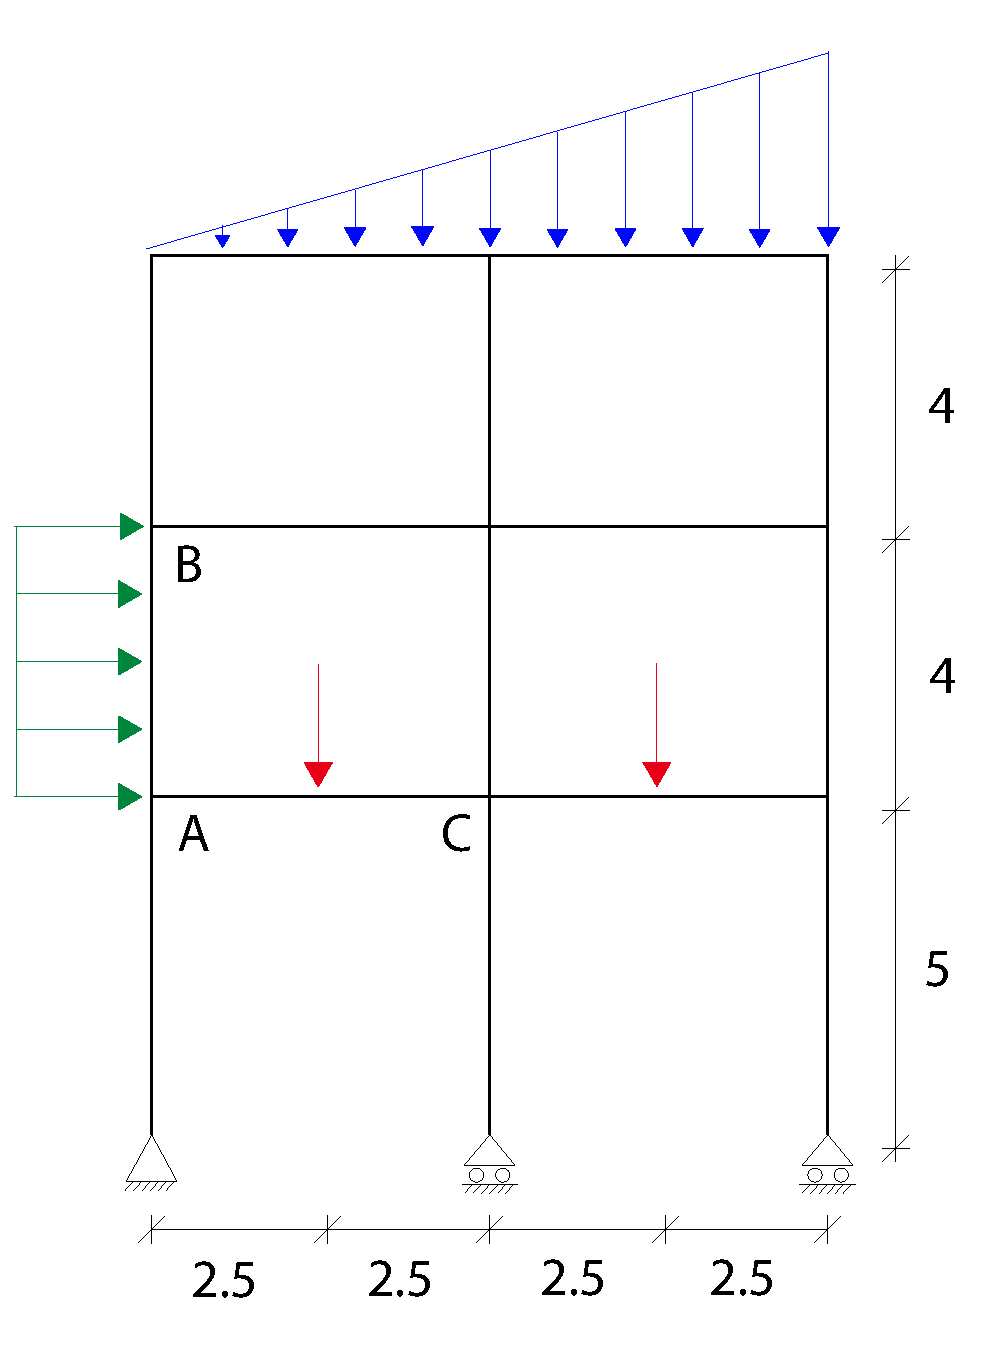
\includegraphics[width=\textwidth]{RecortePuntuable}
\caption{Croquis del pórtico}
\label{fig:croquis}
\end{minipage}
\hspace{0.5cm}
\begin{minipage}[b]{0.4\linewidth}
    \centering
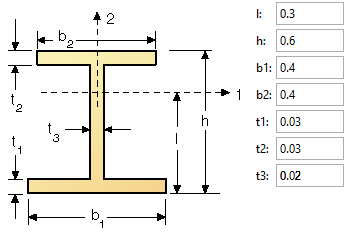
\includegraphics[width=\textwidth]{Figura2.png}
\caption{Perfil viga IPN}
\label{fig:IPN}
\end{minipage}
\end{figure}


\hrulefill
\vspace{4mm}

%%% end of the header

\shufflegroup{test1}
\insertgroup{test1}

%\AMCcleardoublepage    
\clearpage

\AMCformBegin    

%%% beginning of the answer sheet header

\noindent\AMCcode{nummat}{2}\hspace*{\fill}
\begin{minipage}{.7\linewidth}
$\longleftarrow{}$ Escriba su número de matrícula marcando los dígitos
en los recuadros (con ceros a la izquierda si el número es de menos de dos dígitos) y el nombre y apellidos debajo.

\vspace{3ex}

\namefield{\fbox{
   \begin{minipage}{.9\linewidth}
     Apellidos, Nombre:

     \vspace*{.5cm}\dotfill
     \vspace*{1mm}
   \end{minipage}
 }}
\end{minipage}

\begin{center}
 \bf\em Debe dar las respuestas exclusivamente en esta hoja (las respuestas en las demás hojas no serán tenidas en cuenta).
\end{center}

%%% end of the answer sheet header


\AMCform    

\AMCcleardoublepage    

}  

\end{document}
